\hyperdef{}{tilda}{}

\subsection{\texorpdfstring{{Allgemeines zu
Python}}{Allgemeines zu Python}}

\subsubsection{\texorpdfstring{{Herkunft}}{Herkunft}}

\href{http://python.org}{Python}

\begin{itemize}
\itemsep1pt\parskip0pt\parsep0pt
\item
  {wurde Anfang der 1990er Jahre von Guido van Rossum entwickelt}
\item
  {erhielt seinen Namen in Anspielung auf die Monty Pythons}
\item
  {erschien 1994 in der ersten Version 1.0}
\item
  {erschien 2000 in der Version 2.0, die viele Neuerungen enthielt}
\item
  {erschien 2008 in der Version 3.0, die nicht mehr kompatibel mit 2.0
  ist, eine Vielzahl von Verbesserungen aufweist und von uns verwendet
  wird}
\end{itemize}


\subsubsection{\texorpdfstring{{Charakteristik}}{Charakteristik}}

\href{http://python.org}{Python}

\begin{itemize}
\itemsep1pt\parskip0pt\parsep0pt
\item
  {ist eine universelle, interpretierte höhere Programmiersprache}
\item
  {ist sehr stark auf gute Lesbarkeit ausgerichtet}
\item
  {relativ einfach zu erlernen}
\item
  {sehr flexibel (unterstützt objektorientierte und funktionale
  Programmierung)}
\item
  {bietet in der Version 3 endlich eine volle Unicode-Unterstützung}
\item
  {besticht durch einfache Syntax und relativ wenige Schlüsselwörter}
\item
  {ist eine wunderschöne Sprache}
\end{itemize}


\subsubsection{\texorpdfstring{{Installation}}{Installation}}

\begin{itemize}
\itemsep1pt\parskip0pt\parsep0pt
\item
  {Download unter \url{http://python.org} (wir verwenden ausschließlich
  Python 3 im Rahmen des Seminars!)}
\item
  {Installationsanleitung unter
  \url{https://www.python.org/about/gettingstarted/}}
\item
  {die Installation sollte generell problemlos auf fast allen
  Plattformen verlaufen}
\end{itemize}

\subsection{\texorpdfstring{{Bibliotheken und
Entwicklertools}}{Bibliotheken und Entwicklertools}}

\subsubsection{\texorpdfstring{{Allgemeines}}{Allgemeines}}

\href{http://de.wikipedia.org/wiki/Programmbibliothek}{Wikipedia} zur
``Programmbibliothek'':

\begin{quote}
Eine Programmbibliothek bezeichnet in der Programmierung eine Sammlung
von Programmfunktionen für zusammengehörende Aufgaben. Bibliotheken sind
im Unterschied zu Programmen keine eigenständig lauffähigen Einheiten,
sondern Hilfsmodule, die Programmen zur Verfügung gestellt werden.
\end{quote}

\vspace{0.5cm}\par\noindent\textbf{Installation von Python-Bibliotheken mit\vspace{0.5cm}
\href{http://pypa.io}{pip}}

Die Installation von Python-Bibliotheken ist relativ einfach, wenn man
auf das Installationstool \emph{pip} (``pip installs packages'')
zurückgreift. Dieses ist bei den neuesten Pythonversionen (3.4) bereits
vorinstalliert, und kann daher direkt verwendet werden. Die verwendung
ist denkbar einfach. In der Kommandozeile (``cmd'' in der Suchleiste bei
Windows eingeben) gibt man einfach Folgendes ein:

\begin{verbatim}
$ pip install packagename
\end{verbatim}

Daraufhin wird die Bibliothek dann installiert.

\subsubsection{Empfohlene Python-Bibliotheken}
\begin{itemize}
\itemsep1pt\parskip0pt\parsep0pt
\item
  {\href{http://numpy.org}{NumPy}, ``Numeric Python'',
  \url{http://numpy.org}: Sehr gute Bibliothek, die eine Vielzahl
  effizienter numerischer Berechnungen erlaubt und häufig als Grundlage
  für weitere Bibliotheken gefordert wird. }
\item
  {\href{http://scipy.org}{SciPy}, ``Scientific Python'',
  \href{http://scipy.org}{http:/scipy.org}: Sehr wichtige (leider etwas
  langsame) Bibliothek für wissenschaftliche Programmierung. }
\item
  {\href{http://matplotlib.org}{Matplotlib},
  \url{http://matplotlib.org}: Exzellente Bibliothek für das Erstellen
  hochwertiger Plots von Daten.}
\item
  {\href{http://networkx.org}{Networkx}, \url{http://networkx.org}: Sehr
  gute Bibliothek für Netzwerkkalkulationen.}
\item
  {\href{http://lingpy.org}{LingPy}, ``Linguistic Python'',
  \url{http://lingpy.org}: Bibliothek zur Durchführung von quantitativen
  Analysen in der historischen Linguistik (Download unter:
  \url{https://github.com/lingpy/lingpy/releases/tag/v2.4.1-alpha}).}
\end{itemize}


\subsubsection{\texorpdfstring{{Empfohlene
Entwicklertools}}{Empfohlene Entwicklertools}}

\begin{itemize}
\item
  {\href{http://ipython.org}{IPython}, \url{http://ipython.org}: Sehr
  gutes Kommandozeileninterpreter für Python, der vor allem auch das
  Testen von Code ungemein erleichtert. }
\item
  {Installation unter Windows (kann etwas kompliziert werden, aber Sie
  sollten das schon schaffen!):
  \url{http://ipython.org/ipython-doc/2/install/install.html\#windows}}
\item
  {Installation unter Linux/Ubuntu: }

\begin{verbatim}
$ sudo apt-get install ipython3
\end{verbatim}
\item
  {Installation unter Archlinux: }

\begin{verbatim}
$ sudo pacman -S ipython
\end{verbatim}
\end{itemize}

\subsection{\texorpdfstring{{Ein erstes
Programmierbeispiel}}{Ein erstes Programmierbeispiel}}

\subsubsection{\texorpdfstring{{Das Problem}}{Das Problem}}

\begin{quote}
Karlheinz, ein Düsseldorfer Student der Lingustik im 20. Semester, hat
auf einer Mediziner-Party in Köln eine Medizinstudentin kennengelernt,
die ihr Physikum bereits abgeschlossen hat, und möchte sie gerne
wiedersehen. Dummerweise kann er sich jedoch nicht mehr genau daran
erinnern wie sie heißt. Ihr Nachname klang irgendwie nach {{[}maiɐ{]}},
und ihr Vorname war irgendwas in Richtung {{[}krɪstiːnə{]}}, jedoch weiß
er nicht, welche Schreibung er zugrunde legen soll.
\end{quote}



\begin{quote}
Zufällig hat er eine Liste mit den wirklichen Namen und den
dazugehörigen Facebook-Namen von allen Bürgern aus Köln und Umgebung als
Excel-Tabelle auf seinem Computer zu Hause. Wenn er jetzt noch ein
Verfahren finden könnte, das ihm alle Namen anzeigt, die wie
{{[}krɪstiːnə maiɐ{]}} klingen, dann wäre es sicherlich ein Leichtes,
herauszufinden, wo die unbekannte Studentin ihre Tierversuche
veranstaltet, und sie mit einem Pausenkaffee von . Starbucks zwischen
Frosch und Kaninchen zu überraschen\ldots{}
\end{quote}


\subsubsection{\texorpdfstring{{Der Algorithmus}}{Der Algorithmus}}

{ Die Lösung besteht darin, alle Namen, die auf der Liste auftauchen, in
ein anderes Format umzuwandeln, welches den Sprachklang der Wörter
wiedergibt und nicht ihre Schreibung. Ein Algorithmus, der für diesen
Zweck geschaffen wurde, ist die sogenannte ``Kölner Phonetik'' (vgl.
\href{http://bibliography.lingpy.org?key=Postel1969}{Postel 1969}). Die
Kölner Phonetik wandelt Wörter der deutschen Sprache in einen
phonetischen Kode um, mit dessen Hilfe auch Wörter, die unterschiedlich
geschrieben werden, aber gleich klingen, verglichen werden können. So
werden die beiden Namen \emph{Christina Maier} und \emph{Kirsten Mayr}
durch den Algorithmus jeweils in die gleiche Zahlenfolge ``47826-67''
umgewandelt.}



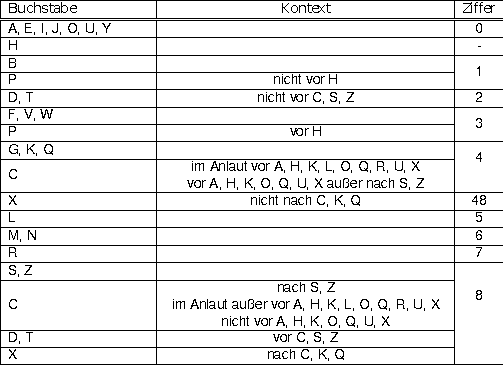
\includegraphics[width=\textwidth]{img/kphon.pdf}


\vspace{0.5cm}\par\noindent\textbf{Das Verfahren}\vspace{0.5cm}

\begin{enumerate}
\itemsep1pt\parskip0pt\parsep0pt
\item
  Wandle jeden Buchstaben schrittweise um und beachte die Kontextregeln.
\item
  Reduziere alle mehrfach hintereinander auftauchenden Ziffern auf eine.
\item
  Entfernen die Ziffer ``0'' an allen Stellen des Wortes, außer am
  Anfang.
\end{enumerate}


\vspace{0.5cm}\par\noindent\textbf{Aufgabe an alle Seminarteilnehmer}\vspace{0.5cm}

Wenden Sie die Kölner Phonetik auf Ihren Vor- und Nachnamen an und
dokumentieren Sie dabei explizit, welche Schritte Sie dabei durchführen.
Warum ist das Verfahren komplizierter, als man am Anfang vermuten
könnte?


\subsubsection{\texorpdfstring{{Die
Python-Implementierung}}{Die Python-Implementierung}}

Die Kölner Phonetik ist in Python von Robert Schindler implementiert
worden und unter der URL (http://pypi.python.org/pypi/kph/0.3)
erhältlich. Wir ignorieren vorerst die Details der Umsetzung und
konzentrieren uns auf die Anwendung. Die Installation ist dank ``pip''
denkbar einfach:

\begin{verbatim}
$ pip install kph
\end{verbatim}

{Die Verwendung auch:}

\begin{verbatim}
>>> import kph
>>> kph.encode("Mattis List")
'628582'
\end{verbatim}

{Aber wie können wir eine lange Liste von Namen abfragen, ohne jeden
Namen einzeln in der Konsole eingeben zu müssen?}

{Richtig, wir brauchen ein Skript!}


\vspace{0.5cm}\par\noindent\textbf{Aufbau von Python-Skripten: Shebang und Kodierung}\vspace{0.5cm}

Die erste Zeile von Python-Skripten sieht oft wie folgt aus:

\begin{verbatim}
#! /usr/bin/env python
# *-* coding:utf-8 *-*

YOUR CODE HERE
\end{verbatim}

Die erste Zeile, die sogenannte
\href{http://de.wikipedia.org/wiki/Shebang}{Shebang line}, erlaubt es,
das Programm durch Doppelklick in Linux- und Mac-Systemen (``unixoide
Systeme'') auszuführen. Die zweite Zeile legt die Kodierung fest und
erlaubt es, bei der Verwendung von Python-2 Programmen, alle Arten von
nicht-ASCII Zeichen zu verwenden. Streng genommen brauchen wir aber
keine der Funktionen, da wir Programme auf Unix-Computern auch leicht
über die Konsole ausführen können, und Python3 UTF-8 voll unterstützt.



\vspace{0.5cm}\par\noindent\textbf{Aufbau von Python-Skripten: Kommentare}\vspace{0.5cm}

\begin{verbatim}
# Dies ist eine Kommentarzeile,
# durch welche es möglich ist, Dinge in das
# Programm zu schreiben, die nachher
# nicht ausgeführt werden.

# Man kann Kommentare Überall einsetzen, man 
# muss aber beachten, dass, wenn man
# sie einsetzt, alles was hinter dem Kommentar-Zeichen folgt, nicht mehr
# interpretiert wird.

1 + 1 # wird hier interpretiert
# 1 + 1 wird nicht interpriert
1 + # ruft einen Fehler hervor, weil das "+" ohne Gegenstück ist
\end{verbatim}

\begin{verbatim}
"Alternativ kann man Dinge auch in Anführungsstriche setzen."

"""
Sicherer ist es allerdings, drei Anführungsstriche auf
einmal zu verwenden, weil man dann auch Anführungsstriche
inerhalb des Kommentars benutzen kann, bzw. auch über
mehrere Zeilen hinweg schreiben kann.
"""
\end{verbatim}



\vspace{0.5cm}\par\noindent\textbf{\href{code/hallo_welt.py}{Die Print-Funktion}}\vspace{0.5cm}

\begin{verbatim}
# file: hallo_welt.py
print("Hallo Welt!")
\end{verbatim}

\begin{verbatim}
$ python3 hallo_welt.py
Hallo Welt!
\end{verbatim}

\vspace{0.5cm}\par\noindent\textbf{\href{code/test_kph.py}{Einbinden von Modulen (Bibliotheken)}}\vspace{0.5cm}

\begin{verbatim}
# file: test_kph.py

import kph 
# importiert die Kölner Phonetik, vorher kann man
# die Bibliothek nicht verwenden

print(kph.encode('Monty Python'))
\end{verbatim}

\begin{verbatim}
$ python3 test_kph.py
662126
\end{verbatim}



\vspace{0.5cm}\par\noindent\textbf{Einige kurze Ideen zum Experimentieren und Nachdenken}\vspace{0.5cm}

\begin{enumerate}
\itemsep1pt\parskip0pt\parsep0pt
\item
  {Experimentieren Sie mit der Kölner Phonetik. Welche Ausgaben erhalten
  Sie, wenn Sie}

  \begin{itemize}
  \itemsep1pt\parskip0pt\parsep0pt
  \item
    {eine Zahl in Anführungsstrichen,}
  \item
    {eine Zahl ohne Anführungsstriche, oder}
  \item
    {Buchstaben mit diakritischen Zeichen (``áłň'') eingeben?}
  \end{itemize}
\item
  {Gibt man statt
  \verb|"Kirsten"|,\verb|"Maier"|
  die Zeile \texttt{encode("Kirsten\ Maier")} ein, verändert sich die
  Ausgabe. Woran liegt das?}
\item
  {Was brauchen wir (welche Routinen, Verfahren), um alle Daten aus der
  Excel-Tabelle von Karlheinz einlesen und in ihre Werte entsprechend
  der Kölner Phonetik umwandeln zu können?}
\end{enumerate}


